\documentclass[10pt,a4paper]{article}
% Copyright (c) 2012 Cies Breijs
%
% The MIT License
%
% Permission is hereby granted, free of charge, to any person obtaining a copy
% of this software and associated documentation files (the "Software"), to deal
% in the Software without restriction, including without limitation the rights
% to use, copy, modify, merge, publish, distribute, sublicense, and/or sell
% copies of the Software, and to permit persons to whom the Software is
% furnished to do so, subject to the following conditions:
%
% The above copyright notice and this permission notice shall be included in
% all copies or substantial portions of the Software.
%
% THE SOFTWARE IS PROVIDED "AS IS", WITHOUT WARRANTY OF ANY KIND, EXPRESS OR
% IMPLIED, INCLUDING BUT NOT LIMITED TO THE WARRANTIES OF MERCHANTABILITY,
% FITNESS FOR A PARTICULAR PURPOSE AND NONINFRINGEMENT. IN NO EVENT SHALL THE
% AUTHORS OR COPYRIGHT HOLDERS BE LIABLE FOR ANY CLAIM, DAMAGES OR OTHER
% LIABILITY, WHETHER IN AN ACTION OF CONTRACT, TORT OR OTHERWISE, ARISING FROM,
% OUT OF OR IN CONNECTION WITH THE SOFTWARE OR THE USE OR OTHER DEALINGS IN THE
% SOFTWARE.

%%% LOAD AND SETUP PACKAGES

\usepackage[margin=0.75in]{geometry} % Adjusts the margins
\usepackage{multicol} % Required for multiple columns of text
\usepackage{mdwlist} % Required to fine tune lists with a inline headings and indented content
\usepackage{tikz}
\usepackage{graphicx}
\usepackage{relsize} % Required for the \textscale command for custom small caps text
\usepackage{hyperref} % Required for customizing links
\usepackage{xcolor} % Required for specifying custom colors
\usepackage{tgpagella} % Use the TeX Gyre Pagella font throughout the document
\usepackage[T1]{fontenc}
\usepackage{microtype} % Slightly tweaks character and word spacings for better typography

\definecolor{dark-blue}{rgb}{0.15,0.15,0.4} % Defines the dark blue color used for links
\hypersetup{colorlinks,linkcolor={dark-blue},citecolor={dark-blue},urlcolor={dark-blue}} % Assigns the dark blue color to all links in the template

\pagestyle{empty} % Stop page numbering

%----------------------------------------------------------------------------------------
%	DEFINE STRUCTURAL COMMANDS
%----------------------------------------------------------------------------------------

\newenvironment{indentsection} % Defines the indentsection environment which indents text in sections titles
{\begin{list}{}{\setlength{\leftmargin}{\newparindent}\setlength{\parsep}{0pt}\setlength{\parskip}{0pt}\setlength{\itemsep}{0pt}\setlength{\topsep}{0pt}}}{\end{list}}

\newcommand*\maintitle[2]{\noindent{\LARGE \textbf{#1}}\ \ \ \emph{#2}\vspace{0.3em}} % Main title (name) with date of birth or subtitle

\newcommand*\roottitle[1]{\subsection*{#1}\vspace{-0.3em}\nopagebreak[4]} % Top level sections in the template

\newcommand{\headedsection}[3]{\nopagebreak[4]\begin{indentsection}\item[]\textscale{1.1}{#1}\hfill#2#3\end{indentsection}\nopagebreak[4]} % Section title used for a new employer

\newcommand{\headedsubsection}[3]{\nopagebreak[4]\begin{indentsection}\item[]\textbf{#1}\hfill\emph{#2}#3\end{indentsection}\nopagebreak[4]} % Section title used for a new position

\newcommand{\bodytext}[1]{\nopagebreak[4]\begin{indentsection}\item[]#1\end{indentsection}\pagebreak[2]} % Body text (indented)

\newcommand{\inlineheadsection}[2]{\begin{basedescript}{\setlength{\leftmargin}{\doubleparindent}}\item[\hspace{\newparindent}\textbf{#1}]#2\end{basedescript}\vspace{-1.7em}} % Section title where body text starts immediately after the title

\newcommand*\acr[1]{\textscale{.85}{#1}} % Custom acronyms command

\newcommand*\bull{\ \ \raisebox{-0.365em}[-1em][-1em]{\textscale{4}{$\cdot$}} \ } % Custom bullet point for separating content

\newlength{\newparindent} % It seems not to work when simply using \parindent...
\addtolength{\newparindent}{\parindent}

\newlength{\doubleparindent} % A double \parindent...
\addtolength{\doubleparindent}{\parindent}

\newcommand{\breakvspace}[1]{\pagebreak[2]\vspace{#1}\pagebreak[2]} % A custom vspace command with custom before and after spacing lengths
\newcommand{\nobreakvspace}[1]{\nopagebreak[4]\vspace{#1}\nopagebreak[4]} % A custom vspace command with custom before and after spacing lengths that do not break the page

\newcommand{\spacedhrule}[2]{\breakvspace{#1}\hrule\nobreakvspace{#2}} % Defines a horizontal line with some vertical space before and after it
\hyphenation{Some-long-word}
\begin{document} 

\maintitle{
\includegraphics[scale=0.03]{../appicon.jpg} Alain Galvan}
\noindent\href{mailto:hi@Alain.xyz}{Hi@Alain.xyz}\bull
\textsmaller{+}1 (305) 302-9275 \bull
\href{https://alain.xyz}{Alain.xyz} \bull Miami, United States

\spacedhrule{0.9em}{-0.4em}

%---------------------------------------------------------------------------------
%	SUMMARY SECTION
%---------------------------------------------------------------------------------

\begin{multicols}{2}

\roottitle{To whom it may concern,}

\noindent \textit{I'm a graduate research assistant for \acr{FIU}'s OpenHID Lab, a Human Computer Interaction (\acr{HCI}) lab part of the High Performance Database Research Center (\acr{HPDRC}), where my research focuses on low level graphics programming, in addition to solving graphics related problems for other researchers in the lab. \\ \\ I'm currently pursuing a PhD in Computer Science with a focus in Computer Graphics Software Architecture.} \\

I believe I would be the perfect fit for \acr{AMD}'s Summer Internship position in Orlando, Florida!

\roottitle{Graphics Research}

Every facet of computer graphics fascinates me, from GPU hardware architecture to the low level graphics APIs like Vulkan and WebGL, all the way up to the application layer and building libraries and abstractions. \\

I'm an avid reader of publications from ACM, IEEE, and books like \textit{Physically Based Rendering by Matt Pharr et al.}, \textit{Game Engine Programming by Jason Gregory}, and even transcribed a series of posts on the graphics pipeline into an ebook. 

\vspace{1.3em}

\noindent 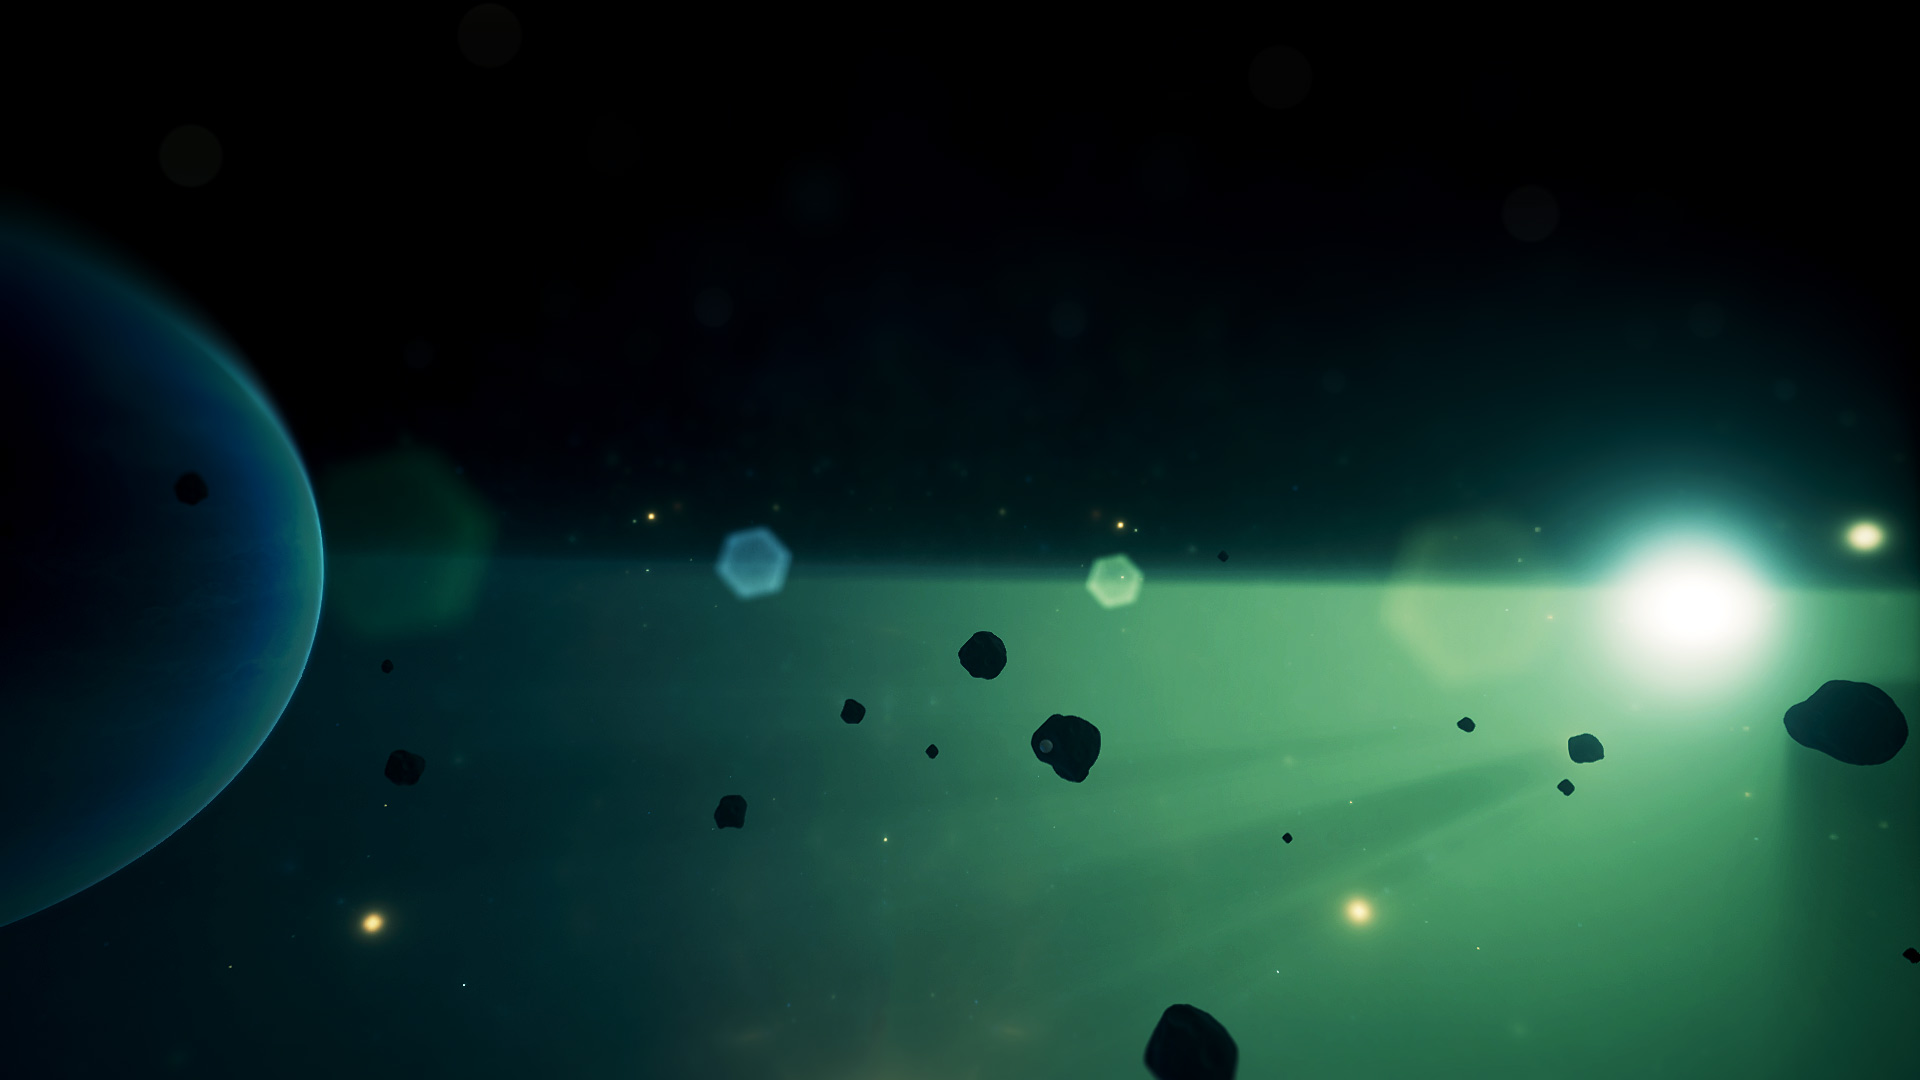
\includegraphics[width=\linewidth]{../portfolio/research/realtime-celestial-rendering/assets/cover.jpg}

\vspace{1.3em}

In the OpenHID Research lab I was always looking for ways to incorporate real time rendering research like Eric Bruneton's Real time atmospheric scattering to the Human Computer Interaction (\acr{HCI}) studies I was responsible for.\\

To that end I've published 2 papers to the \acr{IEEE 3DUI} 2017 Conference in Los Angeles about real-time celestial rendering and the results of a Gesture Elicitation Study focused on 3D environments.


\vspace{1.3em}

\noindent 
\includegraphics[width=\linewidth]{../portfolio/libraries/coronal/assets/cover.jpg}


\vspace{1.3em}

For \textit{Open Source} I've written a \acr{GLTF} Rendering library called \textbf{Coronal} (pictured above), a small TypeScript library that combines Reactive and Functional Programming Techniques with WebGL. 



\vspace{1.3em}

\noindent 
\includegraphics[width=\linewidth]{../portfolio/blog/raw-vulkan/assets/cover.jpg}


\vspace{1.3em}

I published a well received article on writing Vulkan Abstractions that I'm adapting into a tutorial video in the style of \textit{Kurzgesagt - In a Nutshell} titled \textbf{Raw Vulkan}, as well as several other articles on Sound Programming, Game Engine Architecture, Building Web Applications and Much more. \\

I also volunteer! I'm a guitarist, bassist, \& Backup Pianist for The Princeton Church of Homestead, as well as a speaker for \acr{FIU} and the Miami Game Developer Meetup. 

\roottitle{Portfolio \& Contact}

Please visit my Portfolio to see all my work, or check out some of the communities I participate in: \\ \\
\noindent
\noindent \bull Portfolio | \href{https://alain.xyz}{Alain.xyz} \\
\bull Github | \href{https://github.com/alaingalvan}{Github.com/AlainGalvan} \\
\bull LinkedIn | \href{https://linkedin.com/in/alaingalvan}{LinkedIn.com/in/AlainGalvan} \\
\bull Twitter | \href{https://twitter.com/alainxyz}{@Alainxyz} \\
\bull Phone | \textsmaller{+}1 (305) 302-9275

\end{multicols}

\end{document}